% Block diagram of the SIMD vector processing unit.
% Built on its own (standalone) so the same picture is used in the report,
% the README and the video:  tectonic -X compile block_diagram.tex
\documentclass[tikz,border=6pt]{standalone}
\usepackage[T1]{fontenc}
\usepackage{helvet}
\renewcommand{\familydefault}{\sfdefault}
\usetikzlibrary{arrows.meta,fit,backgrounds}

\definecolor{ctrl}{HTML}{CDE2FB}
\definecolor{vec}{HTML}{FBE3D6}
\definecolor{sca}{HTML}{D7F2E6}
\definecolor{mem}{HTML}{EDECE8}
\definecolor{ink}{HTML}{2B2A28}
\definecolor{edge}{HTML}{6F6E69}

\begin{document}
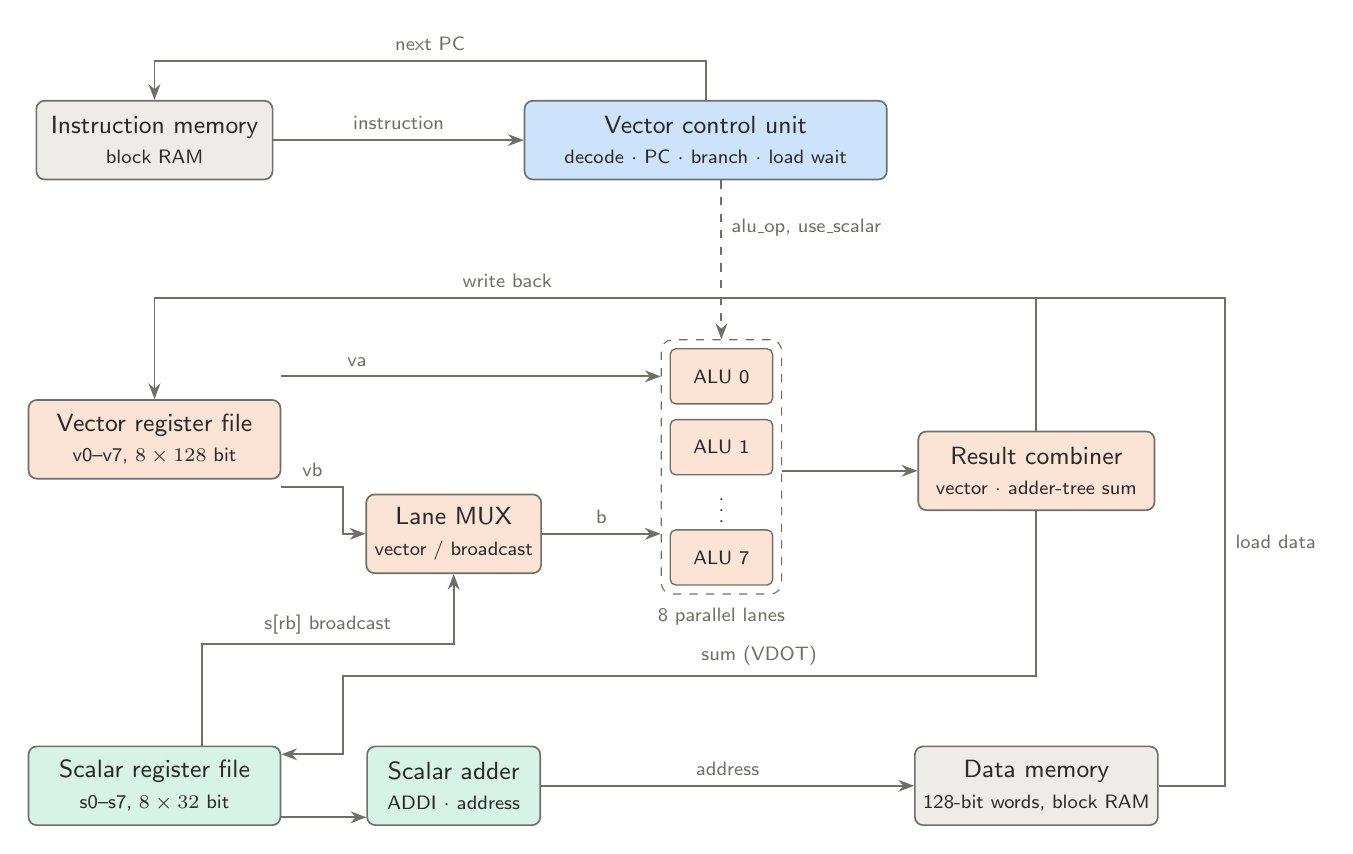
\begin{tikzpicture}[
    x=1mm, y=1mm, font=\small, ink,
    blk/.style={draw=edge, rounded corners=3pt, align=center, minimum height=10mm, inner sep=3pt, line width=0.6pt},
    lane/.style={draw=edge, rounded corners=2pt, fill=vec, minimum width=13mm, minimum height=7mm, font=\scriptsize, line width=0.5pt},
    arr/.style={-{Stealth[length=2mm]}, edge, line width=0.7pt},
    lbl/.style={font=\scriptsize, text=edge}
]

% ---- Blocks (fixed grid) ---------------------------------------------------
\node[blk, fill=mem,  minimum width=30mm] (imem) at (0,8)     {Instruction memory\\\scriptsize block RAM};
\node[blk, fill=ctrl, minimum width=46mm] (ctrl) at (70,8)    {Vector control unit\\\scriptsize decode $\cdot$ PC $\cdot$ branch $\cdot$ load wait};

\node[blk, fill=vec,  minimum width=32mm] (vrf)  at (0,-30)   {Vector register file\\\scriptsize v0--v7, $8\times128$ bit};
\node[blk, fill=vec,  minimum width=22mm] (mux)  at (38,-42)  {Lane MUX\\\scriptsize vector / broadcast};

\node[lane] (l0) at (72,-22) {ALU 0};
\node[lane] (l1) at (72,-31) {ALU 1};
\node[font=\scriptsize] (ld) at (72,-38) {$\vdots$};
\node[lane] (l7) at (72,-45) {ALU 7};
\begin{scope}[on background layer]
  \node[draw=edge, dashed, rounded corners=4pt, fit=(l0)(l7), inner sep=3pt] (lanes) {};
\end{scope}
\node[lbl, below=0.5mm] at (lanes.south) {8 parallel lanes};

\node[blk, fill=vec,  minimum width=30mm] (comb) at (112,-34) {Result combiner\\\scriptsize vector $\cdot$ adder-tree sum};

\node[blk, fill=sca,  minimum width=32mm] (srf)  at (0,-74)   {Scalar register file\\\scriptsize s0--s7, $8\times32$ bit};
\node[blk, fill=sca,  minimum width=22mm] (sadd) at (38,-74)  {Scalar adder\\\scriptsize ADDI $\cdot$ address};
\node[blk, fill=mem,  minimum width=30mm] (dmem) at (112,-74) {Data memory\\\scriptsize 128-bit words, block RAM};

% ---- Fetch loop ----------------------------------------------------------------
\draw[arr] (imem.east) -- node[above, lbl]{instruction} (ctrl.west);
\draw[arr] (ctrl.north) -- ++(0,5) -| node[pos=0.25, above, lbl]{next PC} (imem.north);

% ---- Control signals --------------------------------------------------------
\draw[arr, dashed] (ctrl.south -| lanes.north) -- node[right, lbl, pos=0.3]{alu\_op, use\_scalar} (lanes.north);

% ---- Vector datapath ------------------------------------------------------------
\draw[arr] (vrf.east |- l0) -- node[above, lbl, pos=0.2]{va} (lanes.west |- l0);
\draw[arr] (vrf.east |- 0,-36) -- node[above, lbl]{vb} (24,-36) |- (mux.west);
\draw[arr] (mux.east) -- node[above, lbl]{b} (lanes.west |- mux.east);
\draw[arr] (lanes.east |- comb.west) -- (comb.west);

% ---- Write-back: lane results or loaded data go into a vector register -----
\draw[arr] (comb.north) -- (112,-12) -| node[pos=0.3, above, lbl]{write back} (vrf.north);
\draw[edge, line width=0.7pt] (dmem.east) -- (136,-74) -- node[right, lbl, pos=0.5]{load data} (136,-12) -- (112,-12);

% ---- Scalar side -------------------------------------------------------------------
\draw[arr] (srf.north -| 6,0) -- (6,-56) -- node[above, lbl, pos=0.5]{s[rb] broadcast} (38,-56) -- (mux.south);
\draw[arr] (comb.south) -- (112,-60) -- node[above, lbl, pos=0.4]{sum (VDOT)} (24,-60) -- (24,-70) -- (srf.east |- 0,-70);
\draw[arr] (srf.east |- 0,-78) -- (sadd.west |- 0,-78);
\draw[arr] (sadd.east) -- node[above, lbl]{address} (dmem.west);

\end{tikzpicture}
\end{document}
